\documentclass[conference,a4paper]{IEEE-Template/IEEEtran}

\usepackage{times}
\usepackage[utf8]{inputenc}
\usepackage{booktabs}
\usepackage{tabularx}
\usepackage{graphicx}
\usepackage{ragged2e} 
\usepackage{amssymb}
\usepackage{amsmath}
\renewcommand{\arraystretch}{1.2} 
\usepackage{listings}
% Copyright 2017 Sergei Tikhomirov, MIT License
% https://github.com/s-tikhomirov/solidity-latex-highlighting/

\usepackage{listings, xcolor}

\definecolor{verylightgray}{rgb}{.97,.97,.97}

\lstdefinelanguage{Solidity}{
	keywords=[1]{anonymous, assembly, assert, balance, break, call, callcode, case, catch, class, constant, continue, contract, debugger, default, delegatecall, delete, do, else, emit, event, export, external, false, finally, for, function, gas, if, implements, import, in, indexed, instanceof, interface, internal, is, length, library, log0, log1, log2, log3, log4, memory, modifier, new, payable, pragma, private, protected, public, pure, push, require, return, returns, revert, selfdestruct, send, storage, struct, suicide, super, switch, then, this, throw, transfer, true, try, typeof, using, value, view, while, with, addmod, ecrecover, keccak256, mulmod, ripemd160, sha256, sha3}, % generic keywords including crypto operations
	keywordstyle=[1]\color{blue}\bfseries,
	keywords=[2]{address, bool, byte, bytes, bytes1, bytes2, bytes3, bytes4, bytes5, bytes6, bytes7, bytes8, bytes9, bytes10, bytes11, bytes12, bytes13, bytes14, bytes15, bytes16, bytes17, bytes18, bytes19, bytes20, bytes21, bytes22, bytes23, bytes24, bytes25, bytes26, bytes27, bytes28, bytes29, bytes30, bytes31, bytes32, enum, int, int8, int16, int24, int32, int40, int48, int56, int64, int72, int80, int88, int96, int104, int112, int120, int128, int136, int144, int152, int160, int168, int176, int184, int192, int200, int208, int216, int224, int232, int240, int248, int256, mapping, string, uint, uint8, uint16, uint24, uint32, uint40, uint48, uint56, uint64, uint72, uint80, uint88, uint96, uint104, uint112, uint120, uint128, uint136, uint144, uint152, uint160, uint168, uint176, uint184, uint192, uint200, uint208, uint216, uint224, uint232, uint240, uint248, uint256, var, void, ether, finney, szabo, wei, days, hours, minutes, seconds, weeks, years},	% types; money and time units
	keywordstyle=[2]\color{teal}\bfseries,
	keywords=[3]{block, blockhash, coinbase, difficulty, gaslimit, number, timestamp, msg, data, gas, sender, sig, value, now, tx, gasprice, origin},	% environment variables
	keywordstyle=[3]\color{violet}\bfseries,
	identifierstyle=\color{black},
	sensitive=false,
	comment=[l]{//},
	morecomment=[s]{/*}{*/},
	commentstyle=\color{gray}\ttfamily,
	stringstyle=\color{red}\ttfamily,
	morestring=[b]',
	morestring=[b]"
}

\lstset{
	language=Solidity,
	backgroundcolor=\color{verylightgray},
	extendedchars=true,
	basicstyle=\footnotesize\ttfamily,
	showstringspaces=false,
	showspaces=false,
	% numbers=left,
	numberstyle=\footnotesize,
	numbersep=9pt,
	tabsize=2,
	breaklines=true,
	showtabs=false,
	captionpos=b
}
%\lstset{
%numbers=left,
%numberstyle=\footnotesize,
%stepnumber=1, 
%numbersep=5pt
%}



\usepackage[backend=biber,style=numeric,doi=false,eprint=false,isbn=false]{biblatex}

\usepackage{url}
\setcounter{biburllcpenalty}{7000}
\setcounter{biburlucpenalty}{8000}

\AtEveryBibitem{\clearfield{publisher}}
\AtEveryBibitem{\clearfield{editor}}
% Fix Mendely URL stuff 1
\AtEveryBibitem{\ifentrytype{article}{\clearfield{url}}{}}
\AtEveryBibitem{\ifentrytype{inproceedings}{\clearfield{url}}{}}
\AtEveryBibitem{\ifentrytype{book}{\clearfield{url}}{}}
\AtEveryBibitem{\ifentrytype{incollection}{\clearfield{url}}{}}
% Fix Mendeley URL stuff 2
\DeclareSourcemap{
    \maps{
        \map{ % Replaces '{\_}', '{_}' or '\_' with just '_'
            \step[fieldsource=url,
                  match=\regexp{\{\\\_\}|\{\_\}|\\\_},
                  replace=\regexp{\_}]
        }
        \map{ % Replaces '{'$\sim$'}', '$\sim$' or '{~}' with just '~'
            \step[fieldsource=url,
                  match=\regexp{\{\$\\sim\$\}|\{\~\}|\$\\sim\$},
                  replace=\regexp{\~}]
        }
    }
}

\addbibresource{ref.bib} % Overleaf
%\addbibresource{../../bib/library.bib} % local

\usepackage{todonotes}
\newcommand{\dha}[1]{\todo[linecolor=yellow,backgroundcolor=yellow!25,bordercolor=yellow,inline,caption={}]{Comment by Dominik: #1}}
\newcommand{\todha}[1]{\todo[linecolor=yellow,backgroundcolor=yellow!25,bordercolor=yellow,inline,caption={}]{Todo for Dominik: #1}}
\newcommand{\wjk}[1]{\todo[linecolor=yellow,backgroundcolor=yellow!25,bordercolor=yellow,inline,caption={}]{Comment by Will: #1}}

\begin{document}

\title{Towards Safer Smart Contracts: A Survey of Languages and Verification Methods}



\maketitle

\begin{abstract}
With a market capitalisation of over USD 205 billion in just under ten years, public distributed ledgers have experienced significant adoption.
Apart from novel consensus mechanisms, their success is also accountable to smart contracts. 
These programs allow distrusting parties to enter agreements that are executed autonomously.
However, implementation issues in smart contracts caused severe losses to the users of such contracts.
Significant efforts are taken to improve their security by introducing new programming languages and advance verification methods.
We provide a survey of those efforts in two parts.
First, we introduce several smart contract languages focusing on security features.
To that end, we present an overview concerning paradigm, type, instruction set, semantics, and metering.
Second, we examine verification tools and methods for smart contract and distributed ledgers. 
Accordingly, we introduce their verification approach, level of automation, coverage, and supported languages.
Last, we present future research directions including formal semantics, verified compilers, and automated verification.
\dha{Rewrite this.}
\end{abstract}

\section{Introduction}
%The idea of contracts between independent parties goes back to autonomous agents using a network of agents to solve tasks distributed and based on individual contracts as presented in the contract net protocol ~\cite{Smith1980}.
Smart contracts enable a new generation of decentralised applications.
%Individuals and companies alike invested massively in Initial Coin Offerings (ICOs).
Digital collectibles, autonomous organisations, token funding contracts, gambling platforms, and decentralised exchanges are augmented by smart contracts.
Their success is accountable to a transfer of trust away from individual parties towards the enforced contract logic by a consensus protocol.
Hence, the objective of smart contracts is to minimise the need for trust in peer to peer interactions~\cite{Szabo1997}.
%Smart contracts are programs executed on a blockchain.
The state change of a smart contract is agreed upon by the participants of the consensus protocol of the underlying blockchain.
Thus, their outcome does not rely on a single trusted party but instead on the assumption that a majority or super-majority of consensus participants behaves honestly~\cite{Nakamoto2008,Eyal2014}.
% Significant work focused on creating languages and frameworks for electronic contracts even before the inception of distributed ledgers, for example,~\cite{Andersen2006,Kyas2008,Xu2004}.
% However, distributed ledgers are the ones facilitating the wide-spread adoption of electronic contracts.

Smart contracts combine two unique properties. 
First, anyone can create and publish smart contracts in an open peer to peer system and, second, smart contracts can interact with and manage large amounts of assets.
Contracts are concerned with a range of use cases, including financial services, notaries, games, wallets, or libraries~\cite{Bartoletti2017}.
Further, smart contracts are the enabler of protocols built on top of distributed ledgers, for example, Lightning~\cite{Poon2016}, Plasma~\cite{Poon2017}, Polkadot~\cite{Wood2017}, and TrueBit~\cite{Teutsch2017}.
However, security incidents caused by software bugs lead to severe losses as in the infamous The DAO incident~\cite{Daian2016}, and Parity multi-sig vulnerabilities~\cite{Breidenbach2017Parity,ParityTech2017}. 
%\dha{Include SpankChain example. Maybe also include ERC20 failed to return a value example.}

Substantial efforts are taken to prevent future incidents. 
High-level programming languages are introduced to encourage safe programming practices, for example ~\cite{Hirai2018Bamboo,Ethereum2018Vyper,Schrans2018}.
Languages for distributed virtual machines that allow for easy verification are realised, for example~\cite{Sergey2018,DynamicLedgerSolutions2017,Popejoy2017,Kasampalis2018}.
Tools for analysing source code by symbolic modelling and execution, for example~\cite{Luu2016,Tsankov2017,Kalra2018,Albert2018} as well as formal semantics and verification, for example~\cite{Bhargavan2016,Hildenbrandt2017,Hirai2017}, are developed.

\subsection{Contribution} The number of new languages, approaches for verification, and applicability of verification methods becomes quickly opaque. 
We give a brief technical overview of smart contracts and general security properties in Section~\ref{background}. Due to the practical impact of these approaches to real-world smart contracts, we present a literature survey on current languages and verification efforts.
We contribute an overview of contract language security features including paradigm, instruction set, semantic, and metering in Section~\ref{languages}.
Further, we describe different efforts to verify software including model- and proof-based methods in Section~\ref{verification}. Our overview includes an analysis of the level of automation, coverage, and supported languages.
Last, we introduce directions for future research in Section~\ref{discuss}.

\subsection{Limitations}
This paper focusses on safer smart contracts in relation to smart contract programming language design as well as design and coverage of verification tools.
As such, there are limitations to this survey.
We do not cover aspects related to a developers knowledge of a programming language.
\citeauthor{Delmolino2016} and \citeauthor{DiAngelo2019} present a study on teaching safe smart contract practices~\cite{Delmolino2016,DiAngelo2019}.
Further, we do not cover legal aspects.
Smart contracts and their legal implementations are discussed in~\cite{Neal.2003,Governatori2006,Clack2016}.
Yet, smart contracts do not necessarily have to have a ``real-world'' legal contract equivalent~\cite{Szabo1997,Nakamoto2008,Buterin2013}. 
Projects like Mattereum try to bridge the gap between smart and legal contracts~\cite{Gupta}.
Moreover, we do not cover issues that arise from misaligned incentives.
Smart contracts encode mechanisms that can have explicit or implicit incentives.
The design of these protocols relies on rational agents that behave \emph{truthfully} due to the incentives of the protocol.
This field is closely related to algorithmic mechanism design~\cite{Nisan2007}, however, little work is done combining security and incentive design in the smart contract space.
%Nonetheless, in both settings, the contract languages play a crucial role.

%\subsubsection{Structure} The remainder of our article is structured as follows. Section \ref{background} introduces the background of contracts and languages to express them. We present an overview and a classification of languages in section \ref{languages}. Similarly, verification approaches are examined in section \ref{verification}. Results and future work is discussed in section \ref{discuss}. We conclude in section \ref{conclusion}.

\section{Safer smart contracts}
\label{background}

% Electronic contracts have early beginnings in the AI and agent community where they are used as a basis for interaction \cite{Smith1980}. Moreover, electronic contracts are discussed and used for automating or encoding traditional contracts in organisational and business contexts \cite{Hvitved2010}. Specifically, Ricardian contracts are oft-cited as they introduce encoding natural language contracts into electronic contracts that can be executed by computer systems \cite{Grigg2004}. Later, electronic contracts are applied to enforce agreements between mutually untrusted entities \cite{Szabo1997}.


% If everyone trusted each other, contracts would not be a necessity.
% However, a significant amount of interaction is conducted between untrusted or semi-trusted parties.

\subsection{Contracts and trust}
\dha{Rename to history of smart contracts?}
Contracts are a requirement resulting from an inherent lack of trust between parties.
Electronic contracts have been considered as a way to encode legal contracts (e.g. Ricardian contracts \cite{Grigg2004}) in a Domain Specific Language (DSL). 
They can be processed digitally enabling automated business processes.
How to encode contracts has been surveyed in \cite{Hvitved2010}. 
The author list 13 different requirements that a language needs to fulfil.
He found that those languages can be roughly categorised into four different formalisms including deontic logic, event-condition-action, action-trace, and others.
Most of these languages do not have formal semantics except for \cite{Andersen2006,Kyas2008,Xu2004}.
Underlying those languages is often the assumption that parties adhere to the contract.
Rather than enforcing contracts through a consensus protocol, those systems monitor compliance of participants in the form of norms (permissions, obligations, and prohibitions), e.g.\ \cite{Kyas2008}.

Smart contracts execute agreements on a distributed ledger like Bitcoin or Ethereum \cite{Nakamoto2008,Buterin2013}.
The consensus protocol of the ledger ensures that the smart contract is executed correctly and only results agreed by a majority are accepted.
Consensus protocols enable mutually \emph{distrusting parties} to create contracts and interact.
% Likewise, parties that have a form of \emph{trusted relationship} can utilise smart contracts on a ledger with stronger trust assumptions.
% This can be beneficial since, e.g. transaction rates can be higher and fees (if any) lower.
However, there is a caveat with distributed ledgers and their consensus protocols.
Results of contracts need to be fully deterministic so that each party participating in the consensus protocol reaches the same conclusion with a common set of inputs.

\dha{No unique definition to smart contracts - Ethereum and Bitcoin understanding quite different. Many information is scattered in developments, EIP/BIP, academia.}

% Smart contracts can be used to encode legal contracts, much like the equivalent electronic contract systems \cite{Neal.2003,Governatori2006,Clack2016}.
% Yet, smart contracts do not necessarily have to have a ``real-world'' legal contract equivalent \cite{Szabo1997,Nakamoto2008,Buterin2013}. 
% In the legal context, disputes can be resolved in the traditional legal system of the original contract.
% Where a smart contract does not have a related legal contract, dispute resolution must be included in the protocol of the contract.
% If this is not the case, disputes might not be resolved.
% Projects like Mattereum try to bridge the gap \cite{Gupta}.
% Nonetheless, in both settings, the contract languages play a crucial role.

\subsection{Technical overview}
\dha{Explain the smart contract ``stack''}
Smart contracts need a low-level language that allows deterministic execution. 
A high-level language can make it easier for developers to create new contracts and reason about existing contracts.
In software development, having different sets of languages is a conventional process.
Similarly, we can distinguish three different levels of languages for smart contracts.

\emph{High-level languages} should provide a way to express the desired contracts. These languages can have a wide range of possible paradigms including procedural, logic, functional, or object-oriented. Depending on the use case and intended use of the language, the paradigm can be adjusted. Moreover, multiple high-level languages can exist in parallel to be executed on the same ledger. Examples for high-level languages are Solidity \cite{Ethereum2018Solidity} and Liquidity \cite{OCamlProSAS2018}.

\emph{Intermediary representations (IR)} are between low-level and high-level languages. IRs can be used to write programs to reason about properties (like safety or liveness) or optimising code. Examples include Simplicity \cite{OConnor2017} and Scilla \cite{Sergey2018}.

\emph{Low-level languages} need to implement the contract in a deterministic way so that it can be executed on a distributed virtual machine (VM). Examples include Bitcoin Script \cite{BitcoinWiki2018Script} and EVM bytecode \cite{Wood2014}.

Additionally, the \emph{distributed ledger} plays a vital role in the design of the language. Bitcoin and others implement a UTXO model \cite{Nakamoto2008,Covaci2018}, where contracts are restricted to one transaction. Account-based ledgers have a global state and contracts can typically access this state. 
However, this can introduce security issues when dependencies on the global state are introduced within the contract that can be influenced by parties outside of the contract (typically miners). Other issues revolve around calling into other, possibly faulty or unpredictable, contracts.

\dha{More detail on the ledger? Bitcoin uses \texttt{scriptSig} and \texttt{scriptPubKey} to determine if a tx can be spent. Generally ledger consists of transactions and scripts, consensus protocol, and network protocol.}

\dha{Explain verification efforts. Combination of smart contracts (the logic to be verified) and the ledger environment (the runtime environment).}

\subsection{Security definitions}
\dha{What about a short review about security issues? Desired properties are safety and liveness.}

% \subsection{Contract verification}

%\subsection{Survey objective}
%Smart contracts potentially handle large amounts of money.
%Hence, keeping them safe requires efforts on different levels.
%We summarise the efforts taken to create safe smart contracts by answering the following research question.
%
%\paragraph{\textbf{RQ:}} How can languages and verification methods contribute to safer smart contracts?
%
%
%\paragraph{} In detail, we present relevant previous work according to languages and verification tools.
%High-level languages can encourage secure programming principles that reduce the number of bugs a programmer introduces.
%IR and low-level languages can be designed to simplify program analysis and verification.
%Verification tools can analyse specific properties or full contracts by using representative models or proof methods.
%% Their impact can be promoted by full coverage and ease of use.
%Last, verified compilers are a practice to allow reasoning of programs at a higher level and safe execution at a lower level.
% Design by contract \cite{Meyer1992}

\section{Contract languages}
\label{languages}

Figure \ref{fig:language} gives an overview of smart contract languages.
The approach in (A) is often used to allow program optimisation and verification (e.g. \cite{Lattner2004}). 
Among the projects that follow this approach is Ethereum with Yul \cite{EthereumFoundation2018IULIA}, and Tezos with Liquidity \cite{OCamlProSAS2018} and Michelson \cite{DynamicLedgerSolutions2017}.
Likewise, Scilla is an IR that is targeted by more general languages and compiles down to be executed on a distributed VM \cite{Sergey2018}.

Smart contracts are a comparably new discipline.
Hence, in the early stages, smart contracts were designed as represented by (B).
Bitcoin Script \cite{BitcoinWiki2018Script} requires programmers to write code directly in the low-level stack-based language.
Ethereum, on the other hand, offers multiple high-level languages like Solidity \cite{Ethereum2018Solidity} and Vyper \cite{Ethereum2018Vyper}.
These languages compile directly to EVM bytecode. 

\begin{figure}
\label{fig:language}
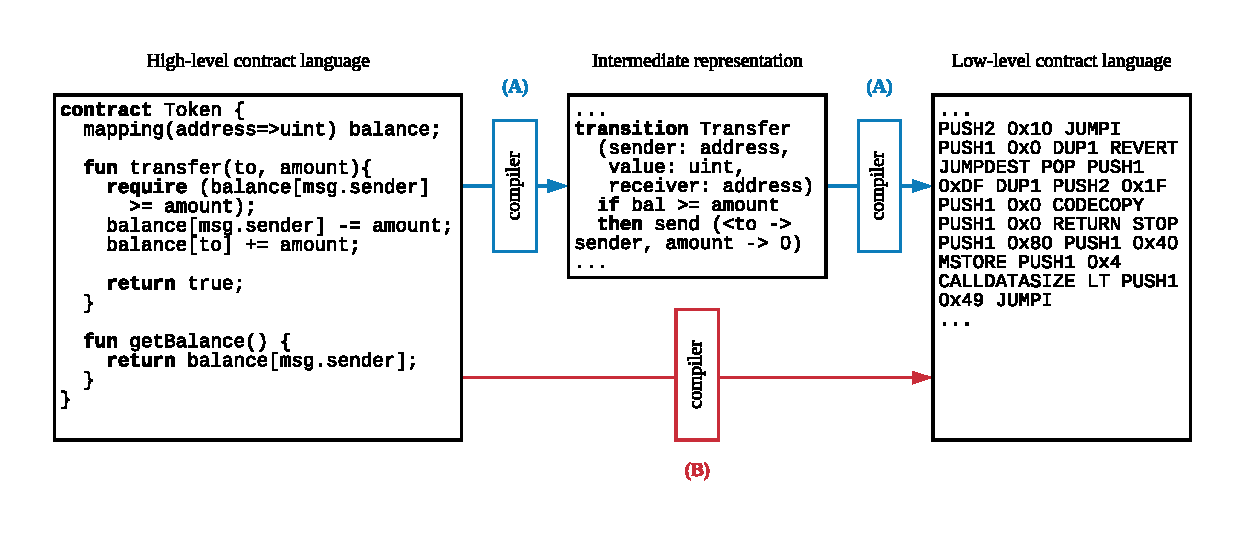
\includegraphics[width=\textwidth]{fig/Language.pdf}
\caption{Different levels of smart contract languages with syntax closely resembled to Solidity (high-level), Scilla (IR), and EVM bytecode (low-evel). (A) represents an optimised version of compiling high-level languages towards the bytecode that allows for example for verification of the IR contract and code optimisations, for example envisioned by \cite{Sergey2018,OCamlProSAS2018}. (B) represents the straightforward compilation from high-level language to bytecode representation as currently employed by Solidity and the EVM \cite{Ethereum2018Solidity,Wood2014}.}
\end{figure}


\subsection{Overview}
The overview we present in table \ref{tab:high-level} is based on five different criteria as listed below. The table gives a general overview. We explain the security properties of the languages within the following subsections.
\begin{itemize}
\item \emph{Type}: We differentiate between high-level, IR, and low-level languages.
\item \emph{Paradigm}: This describes the main paradigm of the language. Note that most languages support multiple paradigms and this criterion is more of an indication of the prevalent paradigm.
\item \emph{Instructions}: The possible instruction set that a language supports can be restricted or Turing-complete.
\item \emph{Semantics}: Languages have a formal or informal semantic. Formal semantics define the exact behaviour of programs written in that language. Informal semantics mostly let the compiler define the exact behaviour.
\item \emph{Metering}: Smart contracts executed on a distributed ledger are re-executed by several nodes. As these computations are costly, metering is a way to charge and limit the execution of a program.
\end{itemize}
\begin{table*}[h]
\centering
\caption{Overview of languages for smart contracts.}
\label{tab:high-level}
\begin{tabularx}{\textwidth}{XXXXXr}
\toprule
\textbf{Language} & \textbf{Paradigm} & \textbf{Instructions} & \textbf{Semantics} & \textbf{Metering} & \textbf{Ref.} \\ \toprule
\textit{Solidity} & object-oriented & Turing-complete & informal\textsuperscript{\dag} & gas, limit & \cite{Ethereum2018Solidity} \\
\textit{Vyper} & procedural & restricted & informal\textsuperscript{\dag} & gas, limit & \cite{Ethereum2018Vyper} \\
\textit{Bamboo} & procedural & Turing-complete & semi\textsuperscript{\dag} & gas, limit & \cite{Hirai2018Bamboo} \\
\textit{Flint} & procedural & Turing-complete & informal & gas, limit & \cite{Schrans2018} \\
\textit{Pyramid Scheme} & functional & Turing-complete & informal & gas, limit & \cite{Burge2018} \\
\textit{Obsidian} & object-oriented & -- & informal & -- & \cite{Coblenz2017} \\
\textit{Rholang} & concurrent & Turing-complete & informal & phlogiston & \cite{Meredith2018} \\
\textit{Liquidity} & functional & restricted & semi\textsuperscript{\dag} & gas, limit & \cite{OCamlProSAS2018} \\
\textit{DAML} & functional & restricted & -- & -- & \cite{Meier2018} \\
\textit{Pact} & functional & restricted & semi\textsuperscript{\dag} & gas, limit & \cite{Popejoy2017} \\
 \midrule
\textit{Simplicity} & pure functional & restricted & formal & -- & \cite{OConnor2017} \\
\textit{Scilla} & functional & restricted & formal & gas, limit & \cite{Sergey2018} \\
\textit{Yul} & procedural & Turing-complete & informal & gas, limit & \cite{EthereumFoundation2018IULIA} \\
%\textit{EthIR} & procedural & Turing-complete & informal & gas, limit & \cite{Albert2018} \\
\textit{IELE} & register-based & Turing-complete & formal & gas, limit & \cite{Kasampalis2018} \\ \midrule
\textit{Bitcoin Script} & stack-based & restricted & informal & script size & \cite{BitcoinWiki2018Script} \\
\textit{EVM} & stack-based & Turing-complete & informal\textsuperscript{\ddag} & gas, limit & \cite{Wood2014} \\
\textit{Bit Machine (Simplicity)} & stack-based & restricted & formal & -- & \cite{OConnor2017} \\
\textit{eWASM} & stack-based & Turing-complete & informal & gas, limit & \cite{EthereumFoundation2018ewasm} \\
\textit{Michelson} & stack-based & restricted & semi\textsuperscript{\dag} & gas, limit & \cite{DynamicLedgerSolutions2017} \\
\bottomrule
\end{tabularx}
\justify
\textsuperscript{\dag} These languages are actively developed. There are efforts to define a formal semantics. \\
\textsuperscript{\ddag} The EVM has been informally defined in \cite{Wood2014}. Formal semantics have been defined afterwards by \cite{Hirai2017,Hildenbrandt2017}.
\end{table*}


\subsection{Languages}

\subsubsection{High-level}
Solidity is the most widely used smart contract language and created for Ethereum \cite{Ethereum2018Solidity}.
Bamboo is designed with formal verification in mind and makes state-transition explicit \cite{Hirai2018Bamboo}. 
Vyper restricts instructions (e.g.\ finite loops and no recursive calls) and prevents other features such as inheritance and overloading \cite{Ethereum2018Vyper}. 
Flint further introduces the definition of function access (by defining the address of the caller) and creates an asset type \cite{Schrans2018}. 
Pyramid Scheme is functional and imperative promoting separation of state-changing and static functions \cite{Burge2018}.

%High-level languages are proposed for other VMs or independent from the ledger implementation.
Obsidian models contracts as finite state machines (FSM) with explicit state transition functions \cite{Coblenz2017}.
Rholang focusses on concurrency and message-passing with statically typed communication channels \cite{Meredith2018}.
Liquidity has a restricted instruction set and enables formal verification \cite{OCamlProSAS2018}.
Rholang and Liquidity are intended for permissionless distributed ledgers.
DAML is functional and developed for financial applications, primarily on permissioned ledgers \cite{Shaul2018,Meier2018,Lippmeier2018,Huschenbett2018,Bernauer2018,Maric2018,Bleikertz2018,Lochbihler2018,Pilav2018}.
Similar, Pact is designed for the Kadena permissioned blockchain \cite{Popejoy2017}.
Both have a restricted instruction set and with the intention to promote formal verification.

%Several other contract languages are developed outside the context of distributed ledgers. The Business Contract Language supports creating and monitoring legal contracts \cite{Neal.2003,Governatori2006}. Specific DSLs have been created for selected use cases,e.g.\, Quality of Service contracts \cite{Braga2009}.
%Other such languages are based on a form of logic and implemented as a dialect of Prolog, e.g.\ \cite{Michael2010}.
%Further, event calculus with an XML formalisation is used model and track state of contracts \cite{Farrell2004}.
% Last, it is proposed to create a language for each specific use case or user type of a contract based on a general-purpose modelling language \cite{Burge2018DSL}.

\subsubsection{Intermediary}
Simplicity is a pure functional language that places itself as an intermediary representation between a higher level (functional) language and a low-level VM \cite{OConnor2017}. 
%It compiles to a low-level language called Bit Machine. 
% It is built for a UTXO model and is not concerned with the global state of the underlying ledger.
Scilla is functional with an automata-based design using explicit state transition functions and handling for communication patterns \cite{Sergey2018}. 
%The semantics are defined in Coq, and formal verification is one of the primary considerations.
Yul (formerly IULIA and JULIA) is introduced as part of Solidity and its compiler \cite{EthereumFoundation2018IULIA}. 
%The idea is to use it as an IR compilation target for multiple high-level languages and optimisations. Further, Yul aims to target the current (1.0) and planned updated EVM (1.5) as well as eWASM.
EthIR is a decompilation target for EVM bytecode \cite{Albert2018}. 
%Its purpose is making the control and data flow of smart contracts explicit allowing analysis such as symbolic execution to operate on its code. 
IELE is derived from its formal semantics and used as an IR for smart contracts \cite{Kasampalis2018}. 
%The syntax is similar to LLVM and has been designed using the K framework \cite{Rosu2007}.
Scilla, Yul, EthIR, and IELE use an account-based blockchain model. Simplicity is built with a UTXO model in mind.

\subsubsection{Low-level}
% The low-level languages in our survey are stack-based. 
Smart contracts are stored on a distributed ledger in the low-level language to be executed by the distributed VM.
Bitcoin scripts are a sequence of op-codes stored within transactions in the Bitcoin network \cite{BitcoinWiki2018Script}. 
%Hence, these contracts need to be re-written and included in the blockchain once the transaction is spent. 
%Possible contracts are for example Hashed Timelock Contracts (HTLCs) \cite{BitcoinWiki2018HTLC}.
The EVM stores programs in the data field of an address in the Ethereum network \cite{Wood2014}. 
%State changing functions are invoked with sending a transaction to the contract. Non-state changing functions are executed locally and do not use gas. Contract functions in the EVM have a signature that can be called by using the contract's address and its Application Binary Interface (ABI).
eWASM is a proposed successor of the EVM based on a deterministic variant of Web Assembly (WASM) \cite{Wanderer2015,EthereumFoundation2018ewasm}.
Michelson is the low-level language of the Tezos blockchain \cite{DynamicLedgerSolutions2017}. It uses accounts as well but is designed to promote formal verification.
% An exception to the low-level languages stored on the blockchain is Scilla. The blockchain Zilliqa directly stores Scilla contracts on its chain.

\subsubsection{General purpose languages}
Apart from using DSLs for programming smart contracts, projects like Hyperledger Fabric or Neo use general purpose programming languages.
This can have advantages as those languages are already known to potential developers, and verification tools might already exist.
For example, Hyperledger Fabric uses Docker containers with smart contracts (so-called ``chaincode'') written in Go, Java, or Node.js \cite{Cachin2016}. 

However, as these languages are originally not designed for smart contracts the global state of the ledger needs to imported through special functions that are typically not available in these languages.
Moreover, these languages often have support for infinite loops and recursion which are not desirable.
Particular types like assets or units also need to be defined appropriately. 
% This can be achieved by using libraries, but arguably, a developer then has to adjust to the new principles imposed by such a library.

\subsection{Paradigm}
% Apart from the dominant paradigm of the languages listed in table \ref{tab:high-level}, special design decisions were made in the languages.

\subsubsection{Explicit state transitions}
Languages including Scilla, Rholang, Bamboo, and Obsidian as well as interfaces to Solidity \cite{Mavridou2018} represent contracts as finite state machines (FSM) or automata. This concept prevents reentrancy and allows to create explicit state transition function. A transaction that is sent to a contract with the intention to change the state either is successful or raises an exception. Moreover, this principle should prevent any calls to other contracts within a state transition function. A state might end or begin with a message (i.e.\ tail-call), but not have any external calls within the state that may change it unpredictably.
% Also, EthIR presents precise data and control flow that allows building rule-based languages. This supports the security of contracts by allowing verification methods to operate on it.

\begin{lstlisting}[caption={A separation of states represented in Bamboo, where each state represents a different contract at the same address.},label=lst:fsm,language=Solidity]
contract Voting() { ... }
contract VotingClosed() { ... }
contract Result() { ... }
\end{lstlisting}

\subsubsection{Functional programming}
Pyramid Scheme, Vyper, Simplicity, Scilla, and Bamboo as well as Pact and DAML for permissioned chains, use functional programming paradigms. Functions in these languages can be designed to be \emph{atomic} and execute entirely or revert. Also, pure functions can be used to indicate that the local or global state is not affected. Functions can call pure functions, but no other state-changing functions.

\subsubsection{Logic programming}
Logic-based languages are interesting as they closely resemble natural language contracts and have been explored in \cite{Idelberger2016}. Logic languages can be purposely non-deterministic. However, they transfer the burden of determinism to the low-level languages and the compiler.


\subsubsection{Stack-based}
All low-level languages are stack-based. Their low-level implementation makes a manual inspection of contracts cumbersome. Hence, automated tools can help to support such verification efforts. Moreover, decompilers are used to convert the stack into a higher level language.

\subsection{Instruction set}
\subsubsection{Restricted instructions}
Vyper, Liquidity, DAML, Pact, Simplicity, Scilla, Bitcoin Script, and Michelson restrict instructions, whereby Bitcoin Script is likely the most restrictive language (also considering that most op-codes are deactivated in Bitcoin). 
The idea is to prevent unwanted behaviour by restricting the instruction set to the necessary operations.
In practice, infinite loops and recursion would block any node in the network executing the smart contract. Hence, it can be directly restricted by the language.
% The EVM and eWASM, on the other hand, strive for Turing-completeness. While there is a discussion of restricting VMs for security reasons, eWASM is supposed to be backwards compatible with the EVM.

\subsubsection{Tail-calls}
Another critical aspect of the instruction set is the possibility of calling other contracts. Executing code in other contracts can potentially introduce unexpected behaviour leading to unpredictable state changes. State changes can be made explicit by using an FSM or automata principle with \emph{tail-calls}. This principle is also suggested for Solidity \cite{ConsenSys2018Security}.
It offers a possibility to update the state of the contract and prevent potential adversaries to gain access to the contract control flow via reentrancy.

\begin{lstlisting}[caption={Tail calls implemented in Solidity.},label=lst:tail-call,language=Solidity]
function claim(uint id) public {
    require(msg.sender == owner[id]);
    funds[id] = 0;
    msg.sender.transfer(funds[id]);
}
\end{lstlisting}

\subsubsection{External function execution}
The EVM offers the \texttt{call}, \texttt{callcode}, and \texttt{delegatecall} instructions to interact with other contracts. The execution context changes based on the invoked call. When using special types within a function like \texttt{msg.sender} or \texttt{msg.value}, the instruction determines which transaction the types refer to. Moreover, \texttt{delegatecall} grants storage access from the calling contract to the called contract. An adversarial contract might thus change the calling contracts storage (i.e.\ local state) arbitrarily. Hence, these external calls should be restricted, or special communication types handle their correct execution as, e.g.\ in Scilla.


%\subsubsection{Fallback functions}
%If a call to an EVM contract fails due to e.g.\ a wrong function signature, the fallback function in the called contract is executed. 

\subsubsection{Restrict overriding}
Overriding functions can lead to issues when reviewing code as it may not be clear which code is actually executed. Assume two functions as listed below.
\begin{lstlisting}[caption={Function overriding with different inputs.},label=lst:tail-call,language=Solidity]
function transfer(address to, uint amount) {}
function transfer(address from, address to, uint amount) {}
\end{lstlisting}
Both functions should theoretically implement the same behaviour. To prevent ambiguities languages like Vyper prevent function overriding.

\subsubsection{Overflow}
The EVM uses fixed-length integers of at most 256 bits.
Hence, developers typically use libraries (e.g. \texttt{SafeMath}) to prevent or detect overflows.
IELE, on the other hand, uses arbitrary-precision signed integers to prevent overflows altogether.

%\subsubsection{Stack limit}


\subsubsection{Code re-use}
\citeauthor{Pontiveros2018} proposes to re-use EVM code to optimise the space usage of code with a new op-code \cite{Pontiveros2018}. This technique could be applied to reference proven secure code patterns.

\subsection{Semantics}

\subsubsection{Formal semantics}
Bamboo, Liquidity, Michelson, and Pact are planned to have a formal semantics once the languages are officially released.  Simplicity and Scilla have a formal semantics defined in Coq. IELE is defined in $\mathbb{K}$, and its implementation has been derived from the formal semantics.
Low-level languages have been informally defined. In later work, the EVM has been formally defined in $\mathbb{K}$ \cite{Hildenbrandt2017}, Lem \cite{Hirai2017}, and F* \cite{Grishchenko2018}.
As other languages have been informally defined, the correct interpretation of programs is left to the compiler. Creating a formal semantic for a higher-level language can enable the creation of verified compilers for said language and support verification efforts.

\subsubsection{Explicit types}
Flint introduces additional types for declaring assets. Smart contracts typically operate on fungible or non-fungible assets. Instead of using existing types (e.g.\ \texttt{uint}), particular asset types can provide additional safety measures like enforcing updating balances before using a \texttt{call} operation sending the asset.

%\subsubsection{Type casting}

\subsection{Metering}

\subsubsection{Script size limit}
Bitcoin Script uses a maximum script size of 10,000 bytes as a restriction to script complexity. Combined with its restricted instruction set, this enables liveness properties of the network. Merkelized Abstract Syntax Tree (MAST) is a proposal to allow larger scripts without increasing the script size limit \cite{Harding2017}.

\subsubsection{Gas}
The EVM, eWASM, IELE, and Michelson use gas and a gas limit to restrict instructions. Rholang's phlogiston essentially implements the gas concept as well. While this allows for liveness of the network as it restricts denial of service attacks, it also opens possible out-of-gas errors. For example, when a function terminates directly after completing a transfer without updating its state (like an account balance), the function can be invoked again without affecting the balance.
Hence, gas considerations are particularly important with external and untrusted calls.


\subsection{Additional security properties} 
\subsubsection{Contract upgrades}
Code is immutable in distributed ledgers. Hence, patterns using contract registries or \texttt{delegatecall} constructs have emerged to upgrade contracts. However, these patterns introduce problems. An alternative approach that sacrifises liveness for more safety is Hydra \cite{Breidenbach2018}.

\subsubsection{Randomness}
Since any local and global state needs to be deterministic and publicly verifiable in distributed ledgers, it is hard to obtain a source to generate pseudo-random numbers.
Miners can influence block-related parameters like timestamps and hashes. The RANDAO suffers from costly implementation. A proposed solution are verifiable delay functions \cite{Boneh2018}.

\subsubsection{Secrets}
As information needs to be verifiable in distributed ledgers, secrets are hard to implement. Commit-reveal schemes make use of hash functions where a user commits to a value by publishing a public hash of the value. Also, zero-knowledge proofs like zk-SNARKS are used to hide information while keeping them verifiable \cite{Sasson2014}.

\subsubsection{Best practices}
Apart from the features that a language supports, best practices can be applied to prevent unintended behaviours \cite{Wohrer2018,ConsenSys2018Security}.
Moreover, templates can be used to create smart contracts \cite{Clack2016}.


\section{Verification methods}
\label{verification}

Verification approaches are outlined in figure \ref{fig:verification}. 
(A) represents verification efforts that base their analysis on the low-level code that is or will be deployed on the distributed ledger. Those tools include K/KEVM \cite{Hildenbrandt2017}, Lem (with their possible proofs in Coq or Isabelle/HOL) \cite{Hirai2017}, and F* \cite{Bhargavan2016,Grishchenko2018}.
Tools listed in (B) use the low-level code and decompile it into an IR to reason about properties in the contracts like Securify \cite{Tsankov2017}, Mythril \cite{Mueller2018}, Oyente \cite{Luu2016,Albert2018}, ECF \cite{Grossman2017}, and Maian \cite{Nikolic2018}. ZEUS is an exception as it uses a high-level language to compile an IR and is not verifying properties based on the low-level code \cite{Kalra2018}.
(C) describes tools that reason directly on the high-level code. Solidity can be annotated with Why3 statements to reason about the correctness of the contract \cite{Reitwiessner2015Why3}. Oyente can be used as well, but will compile code into an IR. Those methods can help to find bugs in contracts, but since they do not operate directly on the low-level code, they rely on verified compilers to infer properties like safety, correctness, or liveness.


\begin{figure}
\label{fig:verification}
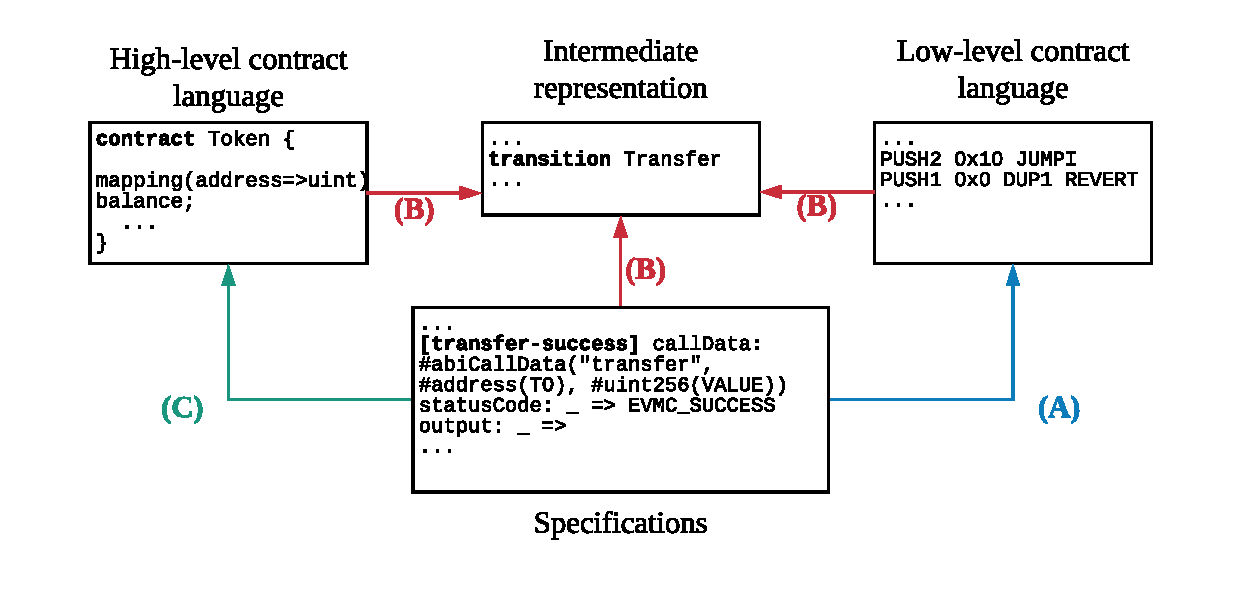
\includegraphics[width=\textwidth]{fig/Verification.pdf}
\caption{Different approaches of verification tools regarding their source for deriving a model or a set of formulas representing the system. Methods listed in (A) directly verify properties from the model or set of formulas from the low-level code. (B) describes tools using an IR from a high-level langauge or from the low-level code to verify the system. Last, (C) describes methods for verifying properties directly from the high-level code.}
\end{figure}

\subsection{Overview}

Verification efforts can be characterised by five criteria \cite[173]{Huth2004}. From these, we adopt three and fixate the other two. 
The application domain concerns smart contracts on a deterministic distributed ledger.
On these ledgers smart contracts are \emph{immutable}, hence, verification before or during, but latest, before deployment, is desirable. Otherwise, they can only be used to find bugs that are already introduced in the software and mostly requires significant efforts to resolve or update the contracts.
Additionally, we included the language that is covered by the specific tool as well as the availability of source code.
This leaves us with the following criteria.
Table \ref{tab:model} presents an overview of the tools we have considered for this survey.

\begin{itemize}
\item \emph{Approach}: In proof-based verification, the system is represented by a set of formulas, while in model-based verification the system is a model. Properties are represented as formulas. The goal is to either proof (proof-based) or to compute whether a model (model-based) satisfies these properties. Proof-based methods typically derive a formal definition of the distributed VM and then try to verify properties of a smart contract. Model-based methods build a model directly from the smart contract and verify the properties with an implicit model of the VM.
\item \emph{Automation}: Fully automated approaches have a set of properties and automatically build a model for the system based on an input (like the source code). Partial automation typically requires defining properties or using a proof-assistant (e.g. Coq or Isabelle/HOL) to define and check proofs.
\item \emph{Coverage}: Property-based verification is concerned with selected parts of the system, while full covers the system as a whole.
\item \emph{Languages}: Lists the languages that are currently, as of September 2018, supported by the methods. Some of the general tools like Lem, F*, K, and Coq can be used for any languages. However, we only list the ones where current research is done.
\item \emph{Source}: Indicates whether the tools and the verification work is available as open source. This criterion is interesting to verify results, experiment with the available tools, and potentially expand them.
\end{itemize}

\begin{table*}
\renewcommand{\arraystretch}{1.3}
\centering
\caption{Overview of model and proof-based verification tools for smart contracts.}
\label{tab:model}
\begin{tabularx}{\textwidth}{XXXXXXr}
\toprule
\textbf{Tool} & \textbf{Approach} & \textbf{Automation} & \textbf{Coverage} & \textbf{Languages} & \textbf{Source} & \textbf{Ref.} \\ \toprule
\emph{Securify} & model & full & full & Solidity, EVM & open & \cite{Tsankov2017} \\
\emph{Mythril} & model & full & property & EVM & open & \cite{Mueller2018} \\
\emph{Oyente} & model & full & property & Solidity, EVM & open & \cite{Luu2016,Albert2018} \\
\emph{ZEUS} & model & full & property & Solidity, Go, Java & closed\textsuperscript{\dag} & \cite{Kalra2018} \\
\emph{ECF} & model & full & property & EVM & open & \cite{Grossman2017} \\
\emph{Maian} & model & full & property & EVM & open & \cite{Nikolic2018} \\ \midrule
\emph{$\mathbb{K}$} & proof & partial & full & EVM, IELE & open & \cite{Hildenbrandt2017,Park2018} \\
\emph{Lem} & proof & partial & full & EVM & open & \cite{Hirai2017,Amani2018} \\
\emph{Coq} & proof & partial & partial\textsuperscript{\ddag} & Scilla, Michelson & open & \cite{Sergey2018,DynamicLedgerSolutions2017} \\
\emph{F*} & proof & partial & partial\textsuperscript{\ddag} & EVM & open & \cite{Bhargavan2016,Grishchenko2018} \\
\bottomrule
\end{tabularx}
\justify
\textsuperscript{\dag} We were not able to find open source code. \\
\textsuperscript{\ddag} Theoretically these tools have a full coverage. However, implementation is as of September 2018 not completed.
\end{table*}




\subsection{Tools}
Model-based methods mostly arise from the need to check contracts for known vulnerabilities. After the DAO and Parity vulnerabilities were known, tools were developed to find similar patterns in other contracts. The proof-based methods arise from the need to proof contracts secure. This requires a formal semantics of the VM and the low-level language. Overall, these methods are used to prevent future vulnerabilities but depend on an exact definition of properties and rigorous formal semantics.

\subsubsection{Model-based}
Securify is a domain-specific model checker for smart contracts \cite{Tsankov2017}. It compiles EVM bytecode to semantics facts and then uses Datalog to define compliance and violation properties to verify the semantic facts. It classifies behaviours of a contract in compliance (matched by compliance properties), violations (matched by violation properties) and warnings (matched by neither). 
Mythril is a symbolic execution of EVM bytecode \cite{Mueller2018}. EVM bytecode is disassembled into a Mythril object, and propositional logic is used to reason about the state space represented as a graph. 
% It is based on the IR LASER \cite{Mueller2018LASER}.
Oyente \cite{Luu2016} and its proposed extension EthIR \cite{Albert2018} build a model from EVM bytecode to verify pre-defined properties. Properties include transaction ordering dependencies, timestamp dependencies, mishandled exceptions, and reentrancy.
ZEUS uses Solidity or Java and Go (as Hyperledger Fabric contracts) as its basis for evaluation \cite{Kalra2018}. It compiles these contracts into an abstract language. Next, properties defined in XACML are used to reason about the contract. The properties together with the abstract language contract get translated to LLVM bitcode for symbolic execution and verification of the properties.
Effectively Callback Free (ECF) objects are a property that is analysed for Ethereum smart contracts\cite{Grossman2017}. A callback method opens up the possibility to change the state of an object (contract) from an external object (contract), which makes reasoning difficult. 
%The authors show that most Ethereum contracts are ECF except for those subject to the vulnerabilities similar to the DAO bug (also referred to reentrancy in other work).
Maian works by symbolic execution of a model of EVM bytecode contracts to find trace vulnerabilities \cite{Nikolic2018}. These vulnerabilities include contracts that leak Ether to unintended parties, can be killed by arbitrary users or lock Ether that cannot be received. 
%They apply their method to verify these properties in real-world contracts.

\subsubsection{Proof-based}
K is a general purpose framework for defining programming languages \cite{Rosu2007}. It is used to build a K representation of the EVM, called KEVM \cite{Hildenbrandt2017}. 
%This VM has been successfully tested against the official test-set of the Ethereum Foundation for any new EVM implementation. 
%Contracts like ERC20 can be specified in K as well \cite{Park2018}. 
A contract can be formally verified using the compiled bytecode, the K contract, and the KEVM virtual machine. Moreover, K is used to defined IELE \cite{Kasampalis2018} and can be used to verify contracts based on this VM.
Lem is used to defining language semantics and can be used to derive implementations in OCaml and enable proof-based verification using Coq, HOL4, or Isabelle/HOL \cite{Mulligan2014}. The EVM has been defined in Lem and subsequently contracts verified using the semantic definition \cite{Hirai2017}. This work is extended by \cite{Amani2018}. 
%The Lem definitions and smart contract verification are pursued by \citeauthor{Hirai2018} at the Ethereum Foundation \cite{Hirai2018}.
Coq is an interactive theorem prover that can be used for any language theoretically. In practice, Scilla is defined in Coq, and there are ongoing efforts to verify Scilla contracts \cite{Sergey2018}. Further, Coq is intended to be used together with the Michelson language \cite{DynamicLedgerSolutions2017}.

\citeauthor{Bhargavan2016} propose to convert Solidity and EVM bytecode to F* \cite{Bhargavan2016}. This can then be used to verify properties in the contract and obtain a secure implementation. However, the work does not present a full implementation.
Further, a complete small-step semantics of the EVM semantics is presented in \cite{Grishchenko2018}. Based on this semantics the authors have implemented in large parts the EVM in F*. F* has then been compiled to OCaml code to verify the EVM implementation against the official Ethereum test suite.

\subsection{Automation} 
Model-based tools are automated. They usually use an SMT solver (e.g. Z3) to explore the fulfilment of violation of properties. Automation offers a significant advantage as the pre-defined properties in the tool can easily be verified on other contracts. Moreover, Securify, Oyente, and Mythril are available as a web-service. This allows developers to check their contracts without the need to install dependencies for model checking locally.

Proof-based tools are partially automated. The Lem, K, F* semantics are focussing on creating the distributed VM that executes the smart contracts. Automation can be reached by defining properties contracts should fulfil. This is partly done by the ERC20 efforts in K and the ``Deed'' contract in Isabelle/HOL. However, it is desirable to define the functionality of a contract and then verify its safety, correctness, and liveness rather than finding selected vulnerabilities. The verification of the properties is then done using an SMT solver (in K) or using an interactive theorem prover (Isabelle/HOL, Coq, F*).

\subsection{Coverage} Most model-based tools verify selected properties. In \cite{Atzei2017} and \cite{Luu2016}, the authors offer a classification of possible vulnerabilities. These vulnerabilities build the basis for the properties to check as the tools try to identify violations or conformance of those patterns to flag a contract as vulnerable.
Model-based tools rely on detecting these properties by static analysis. 
Oyente and Mythril are shown to miss vulnerable patters (false negative) and flag safe contracts as vulnerable (false positive) \cite{Tsankov2017}.
To prevent this, Securify additionally gives a warning if none of its conformance or violation patterns matches.

The desired coverage of proof-based methods is the full contract. 
General smart contract security semantics are formally defined in \cite{Grishchenko2018}. The build a basis for the F* small-step semantics and can be adopted to other general proof-based techniques as well.
However, the security semantics presented are not complete.
Additional, contract specific, properties need to be defined to ensure correctness of the program.
By giving a formal specification of the contract functionalities, a contract can be deemed correct. This approach is beneficial for common standards (e.g. ERC20 or ERC721). A short-coming of proof-based verification is that a verified contract might contain bugs due to incomplete or inaccuracies in the specification or VM semantics \cite{Hirai2016}.

\subsection{Languages} 
%Ethereum is the most popular platform for finding such vulnerabilities. 
%Notably, other languages like Bitcoin Script seem to be quite restrictive leading to less of a need to automatically verify security properties. 
The majority of the tools use the EVM bytecode to derive a model of the contract. ZEUS is an exception as it builds the model based on higher-level languages such as Solidity or Java and Go. Moreover, most models do not implement all EVM opcodes. Hence, vulnerabilities might remain undetected as not all contracts can be fully verified.

Major work efforts are taken in building a formal semantics of the EVM (K, Lem, F*). 
%K and Lem are complete and derived implementations have been tested against the EVM test suite corpus. 
The F* implementation is partially complete. While the EVM semantic is defined after its implementation, IELE, Scilla, and Michelson are designed with formal verification in mind. Hence, their semantics are currently developed and in the future formal verification should be comparably easy. Further, their formal semantics approach helps to build verified compilers.

\subsection{Source} 
All tools have a description in a paper or technical report that gives details about their internals. They offer extensions by creating new properties for verification. Except for Securify and ZEUS, tools can be cloned locally, and additional properties can be added.

The K framework has quite extensive documentation and examples available, followed by the work on Lem and Isabelle/HOL. The Coq and F* methods have been introduced this year, and documentation is yet sparse. Also, the implemented semantics are incomplete making those tools not yet practical to use for smart contract verification.


\section{Research directions}
\label{discuss}

\subsubsection{Compositional specifications}
Current work in specifications focusses on proofing correctness \emph{w.r.t.} to a specification of an entire system or protocol, e.g.~\cite{Pirlea2018}.
However, protocols are often composed of multiple parts, with program logic implemented in several smart contracts and components deployed outside a blockchain.
Future research can focus on two aspects of compositional verification.
First, smart contracts can be verified with built-in defensive programming to handle untrusted code interacting with the contract~\cite{Miller2018smart}.
Defensive programming allows verifying runtime correctness and exception handling of potentially malicious external contract calls.
Second, semantics and models of blockchain systems are primarily monolithic.
Similar to the distinction introduced by \citeauthor{Bonneau2015}~\cite{Bonneau2015}, specifications can focus on separating network, consensus protocol, execution environment, and contract logic.
Verified components can be reused, allowing systems to be modelled and verified more easily.

\subsubsection{Holistic specification}
Formal specifications focusses on verifying properties of individual functions in smart contracts~\cite{Hildenbrandt2017}.
For example, the existing ERC20 formal verification covers the correct execution of functions defined in the standard.
However, a malicious creator of an ERC20 contract could define additional functions to, e.g.\ increase the token balance of individual address or withdraw funds from the contract.
A user of such contract could hardly detect such functions without the high-level language source code.
Even worse, assuming functions are implemented correctly and free of vulnerabilities, neither formal verification nor model checking would flag the contract as incorrect.
Holistic conditions can be created over any function of the contract based on the state variables and accessors to such variables.
% This can be used to verify that the contract does not contain malicious functions.
Model checkers or formal verification tools could then determine that (i) the intended functions can update specific state variables correctly and (ii) the absence of any other function that change state variables (e.g.\ balances or total supply of tokens).
In doubt, a user could verify the necessity of such functions with the creator of a contract before interacting with it.

\subsubsection{Specification language}
Formal verification of smart contracts requires expert knowledge and is usually executed in an interactive theorem proofer like Coq or Isabelle/HOL.
These tools require specialised training and have a steep learning curve.
In order to make verification more accessible to a general audience, DSLs for formulating specifications are created~\cite{He2018,Erfurt2018,RuntimeVerification2018}.
For now, these languages focus on a specific framework.
We imagine that a general specification language for smart contracts could help to make formal verification accessible to a general audience.
Such a language can abstract away some of the underlying complexities of the different blockchains while providing a suitable semantic foundation, for example~\cite{Sergey2018a,Sergey2017}.

%\subsubsection{Verification}
%Verification efforts include categorising and defining security properties for smart contracts, developing model-based tools to verify that contracts are not vulnerable to known bugs, and formal semantics with the intention to prove compliance of a contract implementation to an abstract specification. Proof-based verification requires more effort than model checking for existing vulnerabilities. Hence, verification is sensible for high-value and critical contracts. The Casper contract is currently being formally verified.

%\subsection{Related work}
%\citeauthor{Seijas2017} survey smart contracts for distributed ledger with a focus on Bitcoin, Ethereum, and Nxt \cite{Seijas2017}.
%%They provide an overview of the interactions between smart contracts and the underlying ledger.
%%Further, they sketch selected approaches to create smart contracts and allow for more security.
%In an empirical analysis, the use cases of smart contracts in Bitcoin and Ethereum are discussed\cite{Bartoletti2017}.
%%The authors introduce a taxonomy of smart contracts according to usage categories and design patterns in Ethereum smart contracts.
%The call graph by Ethereum contracts is evaluated in \cite{Frowis2017}.
%%An analysis of security vulnerabilities of smart contracts with a focus on the EVM is presented in \cite{Luu2016} and \cite{Atzei2017}.
%%\citeauthor{Grishchenko2018} extend this work by introducing a formal semantic definition of safety properties of smart contracts.
%
%\citeauthor{Sergey2018} present a brief overview and comparison of 13 smart contracts languages \cite{Sergey2018}. \citeauthor{Tsankov2017} include an overview and comparison to related work on smart contract verification including an evaluation of Securify, Oyente, and Maian \cite{Tsankov2017}.
%
%Apart from language design and verification, other methods are proposed to increase the security of smart contracts. Hydra is a bug-bounty and security protocol for smart contracts \cite{Breidenbach2018}. 
%%The idea is to replicate the contract logic in different implementations that need to reach consensus over state-changing executions and lock contracts if they disagree.
%NECTAR is an extension to Bitcoin's UTXO model and script set \cite{Covaci2018}. 
%%Smart contracts in this setting include a proof about its execution that can be checked to verify correctness.
%Further, game theory and Markov Decision Process (MDP) can be used to model users interacting with a smart contract \cite{Bigi2015}. 
%By applying both methods, the authors validate a protocol build on a smart contract. In that case, external factors like the users are considered explicitly as players in a game.
%
%\subsubsection{Formal semantics and verified compilers}
% The main focus is on developing IRs with formal semantics and creating formal semantics for existing low-level languages. We argue that in the future, more projects need to adopt formal semantics on all language levels to promote verification efforts and prevent ambiguities in compiler implementations. Further, this allows creating verified compilers making it easier to argue about contracts in a high-level language \cite{Hirai2017}. 
%Next, current formal semantics for the EVM combine the VM and the ledger in a single definition. 
%Future work is to separate the semantics for the ledger and the execution environment. 

%\subsubsection{Complete security definitions}
%An initial proposal of formal security definitions is made in \cite{Grishchenko2018}. Those definitions are taken from the perspective of Solidity and the EVM. Hence, more general security definitions for various execution environments are required. Also, it could be interesting to separate the execution environment from the ledger. Moreover, proposed standards like the ERC20 can be formally defined as part of the proposal process. This would allow verifying implementations against a formal specification.

\subsubsection{Automated verification}
During the creation of a smart contract, the code can be annotated or contain explicit statements ensuring runtime correctness.
For example, Solidity from version 5.0.0 offers the conditional statements \texttt{require} and \texttt{assert}.
These conditions are verified during compile time using symbolic execution with SMT-solvers such as Z3 and CVC4~\cite{Alt2018}.
We imagine that other smart contract language compilers could use a similar approach to verify code at compile time.
Smart contract languages can include standardised patterns to declare pre- and postconditions.
Also, the language compilers can be designed to require developers to formulate conditions as part of the contract explicitly.

\subsubsection{Proof-carrying code}
The majority of blockchain systems reaches consensus over a state update $S \rightarrow S'$ by replicating the state transition function executed as part of the transaction. 
As an alternative, proof-carrying smart contracts require provable fulfilment of a specification $\Phi$ on a state transition. 
This has two advantages: First, a state transition can be proven and verified by publishing and subsequently verifying an ideally succinct proof. 
Second, by publishing a specification $\Phi$ of a contract, the contract implementation can be updated verifiably.
When an update of the code (i.e.\ resolving a bug or optimising resource usage) is available, the code can be updated by checking if the update is satisfying $\Phi$.
An example of this approach for ERC20 contracts is introduced in~\cite{Dickerson2018}.
Similarly, ZEXE proposes to use succinct proofs over smart contract transition functions~\cite{Bowe2018}.
However, creating and writing proofs for smart contracts requires expert knowledge.
Future directions for smart contract languages include high-level languages that compile into programs suitable for cryptographic proofs protocols (i.e.\ arithmetic and boolean circuits).
Further, a comparative analysis of different cryptographic schemes (e.g.\ zk-SNARKs, zk-STARKS, or Bulletproofs) and their applicability for smart contract languages is required.


\subsubsection{Economic properties}
A core ability of smart contracts is implementing crypto economic protocols.
Hence, they encode incentive mechanisms that provide incentives to honest parties and penalises misbehaviour.
Formal methods and their tools for smart contracts focus on verifying properties \emph{w.r.t.} safety and liveness.
Future model checkers can be developed to verify the incentive structures of smart contracts.
% Predicates can be formulated over the payout functions of each user type of a contract.
Model checkers simulate different strategies for users of a contract and calculate properties including social welfare and Nash equilibria.
Moreover, they can utilise statistical methods such as Markov chains.

%\subsubsection{Visual representation and programming}
%Visual representations of programs can help to understand and manually verify the control flow. 
%Solgraph and Mythril
%Following the ideas of making general programming accessible to a wide audience~\cite{Resnick2009}, smart contract programming can be made safer and more accessible by using visual programming paradigms.
%Meadow is an example of a visual representation of programs written in the Marlowe smart contracts langauge~\cite{Seijas2018}.


%\subsubsection{Language design}
%High-level languages for smart contracts are designed and improved to promote safe smart contracts.
%This is achieved by making state changes explicit by using an FSM/automata approach. 
%They typically restrict the instruction set by only allowing finite loops and recursion.
%Moreover, the code should be as explicit as possible by preventing function overloading, creating explicit types for assets and units, and promoting pure functions.
%Intermediary languages are developed with formal verification and optimisations in mind.
%This is an attempt to bring best practices from software engineering and language theory to distributed ledgers.
%Low-level languages are built to allow formal verification and at the same time give a run-time optimised execution on a distributed ledger.
%Combining those practices and applying them in the development cycle helps create secure smart contracts.




%\subsubsection{Protocol level verification}
%Formally verified protocols. Example Casper~\cite{Palmskog2018} and consensus protocol~\cite{Pirlea2018}. 


%\subsubsection{Automated verification}

%\subsection{Future work}
%Formal semantics

%Verified compilers

%Automated verification

\section{Conclusion}
\label{conclusion}
An overview of smart contracts and verification methods is presented.
Languages are developed and improved to allow easier verification by defining formal semantics. Also, secure patterns like explicit state transitions and restricted instructions are applied. Verification efforts concentrate on finding known vulnerabilities and formally defining smart contract logic to verify implementations.
We note areas of future work including compositional and holistic specifications, general specification languages for smart contract verification, automated verification approaches built into compilers, proof-carrying smart contracts, and economic models.

%We note three areas of future work. Formal semantics are being adopted for low-level languages, and selected IRs have been designed from a formal semantics. However, high-level languages with full formal semantics are just being developed.
%Formal semantics on all levels of languages is a requirement to develop verified compilers. Verified compilers and formal semantics can then be used to build automated proof-based verification methods.

% Smart contracts are a new type of programs that have direct access to currency and are executed on a globally distributed network. 



\printbibliography

\end{document}
